\documentclass[a4paper]{scrreprt}

% Uncomment to optimize for double-sided printing.
% \KOMAoptions{twoside}

% Set binding correction manually, if known.
% \KOMAoptions{BCOR=2cm}

% Localization options
\usepackage[english]{babel}
\usepackage[T1]{fontenc}
\usepackage[utf8]{inputenc}

% PDF-compatible landscape mode.
% Makes PDF viewers show the page rotated by 90°.
\usepackage{pdflscape}

% Advanced tables
\usepackage{tabularx}

% Fancy tablerules
\usepackage{booktabs}

% Current time
\usepackage[useregional=numeric]{datetime2}

% Float barriers.
% Automatically add a FloatBarrier to each \section
\usepackage[section]{placeins}

% \usepackage{geometry}
% \usepackage{layout}

% Math tools
\usepackage{mathtools}
% Math symbols
\usepackage{amsmath,amsfonts,amssymb}
\usepackage{amsthm}
% General symbols
\usepackage{stmaryrd}

% Utilities for quotations
\usepackage{csquotes}

% Bibliography
\usepackage[
  style=alphabetic,
  backend=biber, % Default backend, just listed for completness
  sorting=ynt % Sort by year, name, title
]{biblatex}
\addbibresource{references.bib}

% Source code & highlighting
\usepackage{listings}

% SI units
\usepackage{siunitx}

\newcommand{\lecture}{41506 - Seminar Cryptography and Data Security}
% Convenience commands
\newcommand{\mailsubject}{\lecture - Report}
\newcommand{\maillink}[1]{\href{mailto:#1?subject=\mailsubject}
                               {#1}}

% Should use this command wherever the print date is mentioned.
\newcommand{\printdate}{\today}

\subject{\lecture}
\title{Punchscan: Digital voting scheme with paper-based receipts}

\author{Michael Senn \maillink{michael.senn@students.unibe.ch} --- 16-126-880}

\date{\printdate}

% Needs to be the last command in the preamble, for one reason or
% another. 
\usepackage{hyperref}

\begin{document}

\maketitle

\begin{abstract}
	Lorem ipsum dolor si amet, et coniunctur.
\end{abstract}

\chapter{Introduction}
\label{chapter:introduction}

In the course of history, many different voting systems have been designed and
used. They differ in their trust models, their usability and other aspects. In
the last decades, ongoing digitalization has also influenced election systems
in that electronic systems have started to play a role in the voting process.

One such system is Punchscan, published in the early 2000s. It is a voting
system using paper ballots, yet heavily relies on cryptographic operations to
provide voter privacy, resilience towards malicious parties, and individual
verifiability. This report aims to provide an overview of Punchscan's
workings and shortcomings.

Chapter \ref{ch:ballot_design_and_voting} will start by discussing the ballot
layout as well as the voting process from the point of view of the voter.
Chapter \ref{ch:setup} will describe the work performed by the election
authority and auditors ahead of time. Chapter \ref{ch:tally} will describe the
tally phase including its audits. Finally chapter \ref{ch:security} will
discuss the integrity and privacy goals --- as well as how and if they are
achieved --- of Punchscan. 

% TODO don't like this sentence
The report is heavily based on the introductory paper to Punchscan by Fisher et
al.\autocite{fisherPunchscanIntroductionSystem2006}, with other work being
referenced where appropriate.

\section{Involved parties}

People participating in the Punchscan election system can be grouped into one
of three categories.
\begin{description}
\item[Voters] Voters participate in the election. They are assumed to be able
to authenticate themselves towards the election authority. Malicious voters may
attempt to learn of others' votes, or sell their own vote to third parties.
\item[Election authority] The election authority consists of a single person
--- or a set of persons in a threshold setting --- which handles the setup and
tally phases of the election. A malicious election authority may attempt to
influence the outcome of the election. In a broader sense the election
authority also includes poll workers assisting voters. The election authority
is assumed to be able to generate key material at will, and share it
securely with other parties where required.
\item[Auditors] Auditors are a set of people tasked with ensuring vote
integrity. At least one auditor is assumed to be honest.
\end{description}

\section{Notation and terminology}

\subsection{Permutations}

Permutations will be denoted by the letter $\pi$, with an index describing
their purpose. As an example, $\pi_{top}$ will be used to refer to the
permutation of the ballot's top page. The standard one-line notation will be
used, where $\pi = cba$ refers to a permutation $\pi$ such that $\pi(a) = c,
\pi(b) = b, \pi(c) = a$. For permutations over two elements the notation from
the Punchscan paper is adopted, where $\rightarrow$ is the identity permutation
and $\circlearrowright$ is the permutation flipping the two elements.
Composition of permutations is denoted as $\pi_1 \circ \pi_2$, evaluated
right-to-left.

\subsection{Representation of data}

The Punchscan system generates and manipulates a fair bit of data, which will
be described in terms of relational databases such as `tables', `rows',
`columns', `primary keys', `foreign keys' and so on. This does not imply a
requirement for specific implementations of Punchscan to use a relational
storage system, although no clear benefit to using non-relational storage is
apparent as the data is inherently relational.

\chapter{Ballot design and voting}
\label{ch:ballot_design_and_voting}

\section{Ballot design}

A Punchscan ballot consists of two pages stacked atop each other, as shown in
figure \ref{fig:punchscan_ballot}. It is uniquely identified by a numerical ID
printed on both pages. The top page contains the questions asked as well as all
possible answers. Each answer is mapped to a symbol --- in this case the
letters `a', `b' and `c'. The bottom page contains the same symbols, which can
be seen through cutouts in the top page when stacked atop each other. Both the
mapping of answers to symbols on the top page, as well as the order of symbols
on the bottom page, are independent random permutations per ballot. Multiple
questions can also be printed on the same ballot without loss of functionality
or privacy, as will be discussed later.

\begin{figure}[h]
\centering
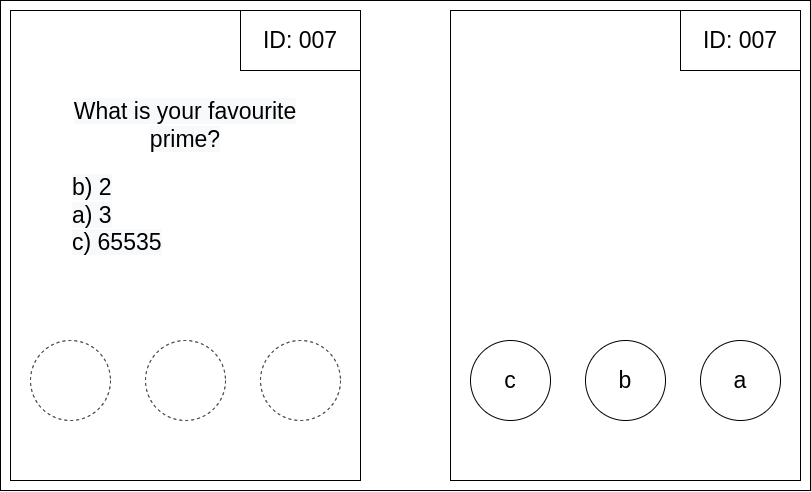
\includegraphics[width=0.7\textwidth]{../resources/high_level_ballot.drawio}
\caption{Punchscan ballot consisting of top (left) and bottom (right) page}
\label{fig:punchscan_ballot}
\end{figure}

\section{Voting process}

After having identified themselves at the polling place, a voter will have to
commit to getting to keep either the top or the bottom page of the ballot as a
receipt. They will then receive a random ballot, consisting of a top and bottom
page stuck together and enter the voting booth.

Within, the voter will read the question and decide on their answer. They will
look up which symbol their choice maps to on the top page, and then look
through which hole on the top page the corresponding symbol printed on the
bottom page is visible. They will then mark the corresponding slot using a
dauber --- a huge highlighter as used in Bingo --- thereby leaving a stain on
both the top as well as the bottom page of the ballot. The effect of having
marked their choice is shown in figure \ref{fig:punchscan_ballot_voted}.

The voter will then destroy the half of the ballot they will not keep by
feeding it through a shredder. They then exit the voting booth, and hand the
remaining half to a poll worker. The poll worker will scan the page, and feed
it through an OCR software. The voter gets to see and confirm that the scanned
page, including the detected choice, matches their physical copy. If so they
get to leave, keeping their scanned half of the ballot as a receipt.

\begin{figure}
\centering
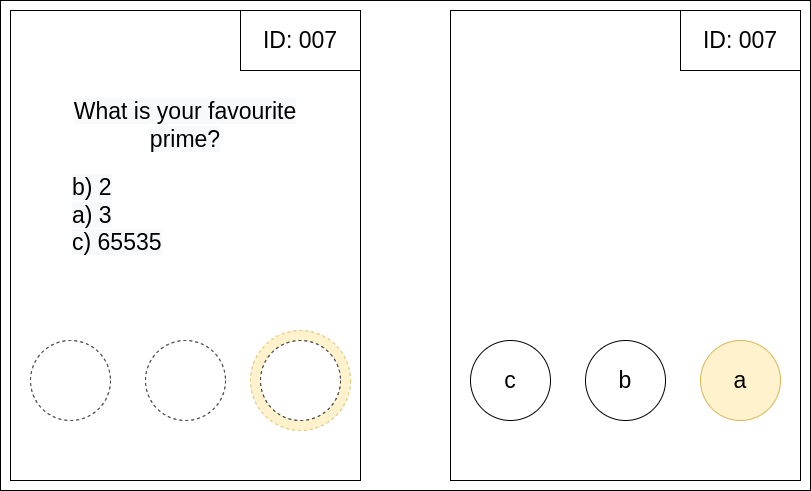
\includegraphics[width=0.7\textwidth]{../resources/high_level_ballot_voted_split.drawio}
\caption{Top (left) and bottom (right) pages of ballot after voter chose `3' as their favourite prime}
\label{fig:punchscan_ballot_voted}
\end{figure}


\printbibliography

\end{document}
